\section{Empirical Results}\label{sec:experiment}

In this section we present the empirical results obtained from running Hash-join, LIP and LIP-$k$ on several datasets. In Section \ref{sec:dataset}, we present the datasets we use and describe how we generate skewed and adversarial datasets. In Section \ref{sec:time} we present the running time of multiple strategies and discuss their performance. In Section \ref{sec:ratio} we discuss how $k$ affects the competitive ratio of LIP-$k$ empirically on our datasets.

\subsection{Datasets}
\label{sec:dataset}

The Star Schema Benchmark (SSB) is a variation of the TPC-H benchmark 
consisting of a large central fact table \texttt{LINEORDER} and four smaller dimension tables (\texttt{DATE}, \texttt{PART}, \texttt{CUSTOMER}, and \texttt{SUPPLIER}).
The benchmark has 13 select-project-join queries split across four groups. 
We generate all tables in the benchmark using the SSB generator found at \url{https://github.com/UWQuickstep/SQL-benchmark-data-generator/tree/master/ssbgen}.
We refer the \texttt{LINEORDER} table produced from the SBB generator with SF = 1 as \texttt{LINEORDER-UNIFORM}, 
since it's foreign keys for each tuple are sampled from a uniform distribution of possible keys ({\it i.e.} there is no skew).

We modify the \texttt{LINEORDER-UNIFORM} table to produce four additional skewed \texttt{LINEORDER} tables.
For simplicity in generating skew tables, we skew the \texttt{ORDER DATE} foreign key in the origin \texttt{LINEORDER} table, corresponding to the primary key of the \texttt{DATE} table. 
We alter the distribution of \texttt{ORDER DATE} foreign keys satisfying \texttt{DATE.YEAR = 1997 OR DATE.YEAR = 1998}, which we shorten to \texttt{SKEW PRED}.
The skewed tables are as follows:


\begin{itemize}
    \item \texttt{LINEORDER-DATE-FIRST-HALF}: Let $N$ be the total number of batches in \texttt{LINEORDER}. 
    The first $N/2$ batches have $\sigma_{\texttt{SKEW PRED}} = 1$ while the remaining $N/2$ batches have $\sigma_{\texttt{SKEW PRED}} = 0$.
    In other words, The first $N/2$ batches contain only keys satisfying \texttt{SKEW PRED}, 
    while the next $N/2$ batches contain only keys not satisying \texttt{SKEW PRED}, 
    and so on. 

    \item \texttt{LINEORDER-DATE-50-50}: The first 50 batches have $\sigma_{\texttt{SKEW PRED}} = 1$ while the next 50 batches have $\sigma_{\texttt{SKEW PRED}} = 0$, and so on.

    \item \texttt{LINEORDER-DATE-LINEAR}: $\sigma_{\texttt{SKEW PRED}}$ increases linearly from 0 to 1 across the \texttt{LINEORDER} table, 
    {\it i.e.} batch $k$ has $\sigma_{\texttt{SKEW PRED}} = k/N$.

    \item \texttt{LINEORDER-DATE-PART-ADVERSARY}: We defer discussion on this dataset to Section~\ref{sec:ratio}, 
    as it requires a careful description of its construction.

\end{itemize} 


All datasets are summarized in Table~\ref{tab:skew_datasets}. All datasets use the same dimension tables originally produced from the SSB generator with SF = 1.

\begin{table}
\begin{center}
\begin{tabular}{ |>{\ttfamily}l|>{\ttfamily}c|l| } 
\hline
{\bf Dataset Name} & {\bf Skewed Foreign Keys} & {\bf Description of Skew} \\
\hline
\hline
LINEORDER-UNIFORM& N/A & No skew. Generated from SSB data generator\\
& & with SF = 1.\\
\hline
LINEORDER-DATE-FIRST-HALF& ORDER DATE & $\sigma_{\texttt{SKEW PRED}}$ changes from 1 to 0 halfway through\\
& &  the table.\\
\hline
LINEORDER-DATE-50-50& ORDER DATE & $\sigma_{\texttt{SKEW PRED}}$ changes from 1 to 0 or from 0 to 1 \\
& & every 50 batches. \\ 
\hline
LINEORDER-DATE-LINEAR& ORDER DATE & $\sigma_{\texttt{SKEW PRED}}$ increases linearly from 0 to 1 \\
& & through the table. \\
\hline
LINEORDER-DATE-PART-ADVERSARY& ORDER DATE & See Section~\ref{sec:ratio}\\
& PART KEY & \\
\hline

\end{tabular}
\end{center}

\caption{Brief descriptions of all datasets studied.}
\label{tab:skew_datasets}
\end{table}

\subsection{Execution Time}
\label{sec:time}

\begin{figure}
    \centering
    \subfloat[]{
        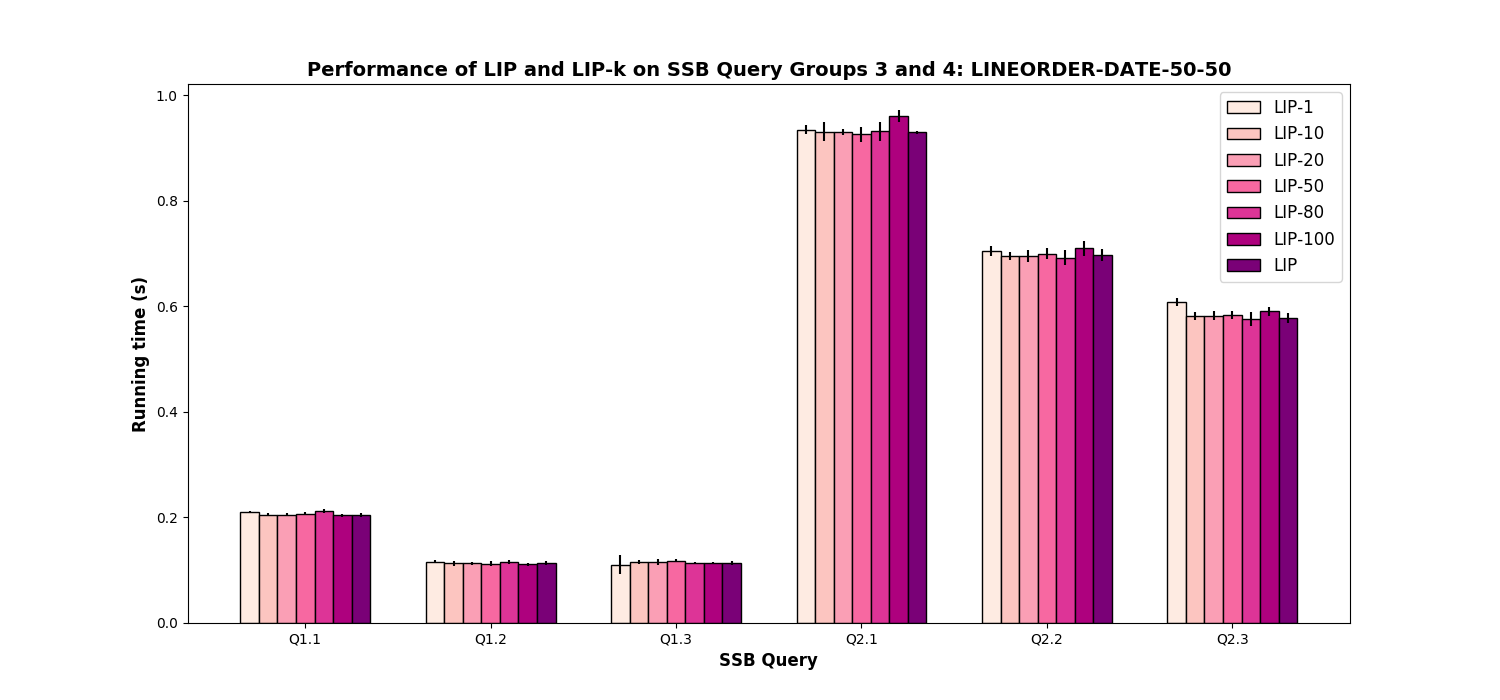
\includegraphics[width=0.9\textwidth,keepaspectratio]{lip-and-lipk-date-50-50-q1-q2}

    }\\
    \subfloat[]{
        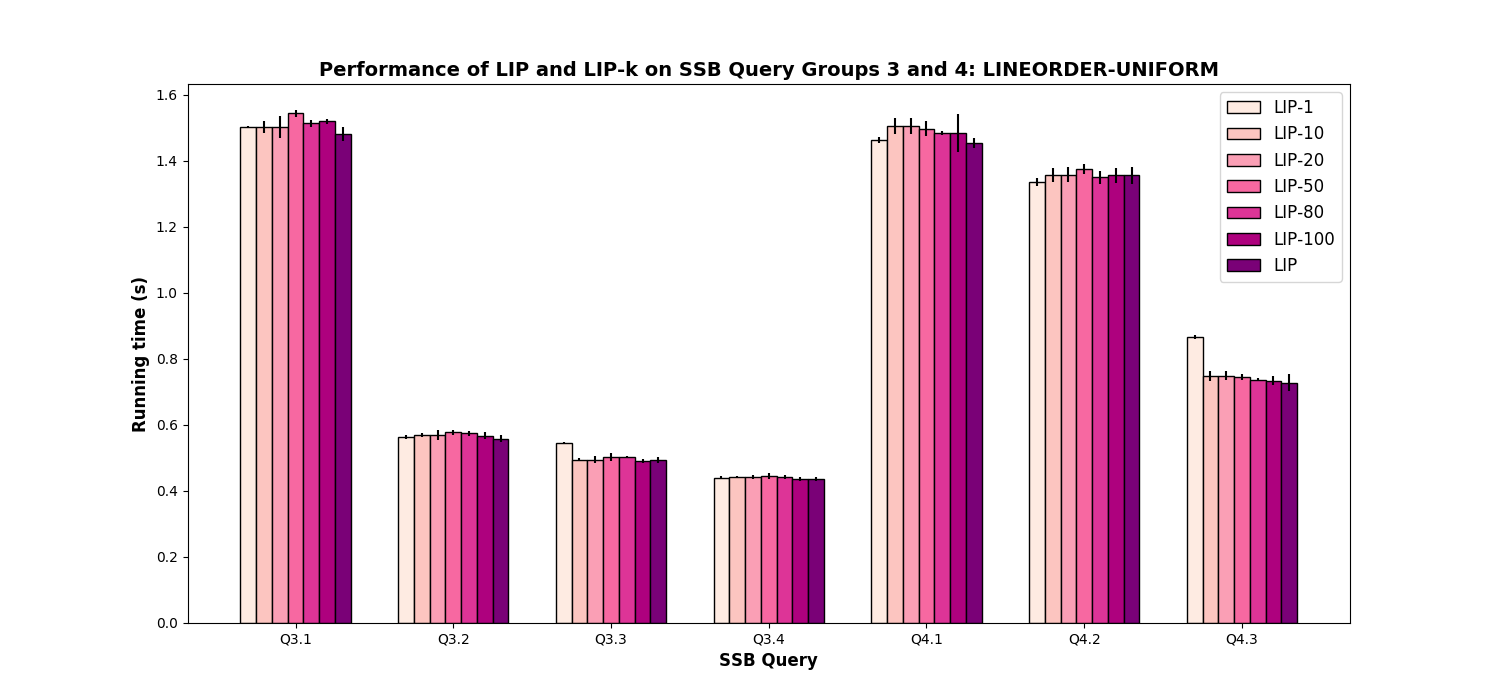
\includegraphics[width=0.9\textwidth,keepaspectratio]{lip-and-lipk-uniform}
    }
    \caption{Execution time for SSB query groups 1 and 2 on (a) \texttt{LINEORDER-DATE-50-50} and query group 3 and 4 on (b)~\texttt{LINEORDER-UNIFORM}}
    \label{fig:times0}
\end{figure}

\begin{figure}
    \centering
    \subfloat[]{
        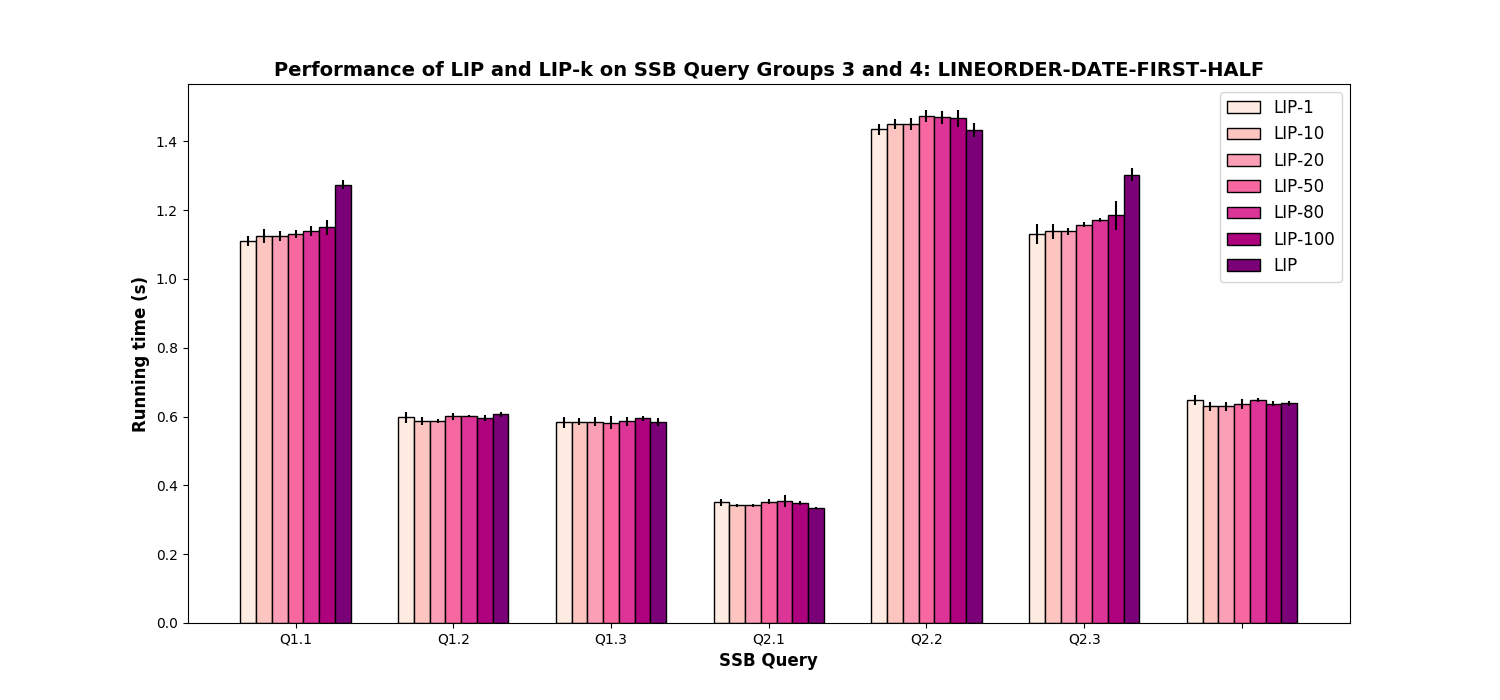
\includegraphics[width=0.9\textwidth,keepaspectratio]{lip-and-lipk-date-first-half}
    }\\
    \subfloat[]{
        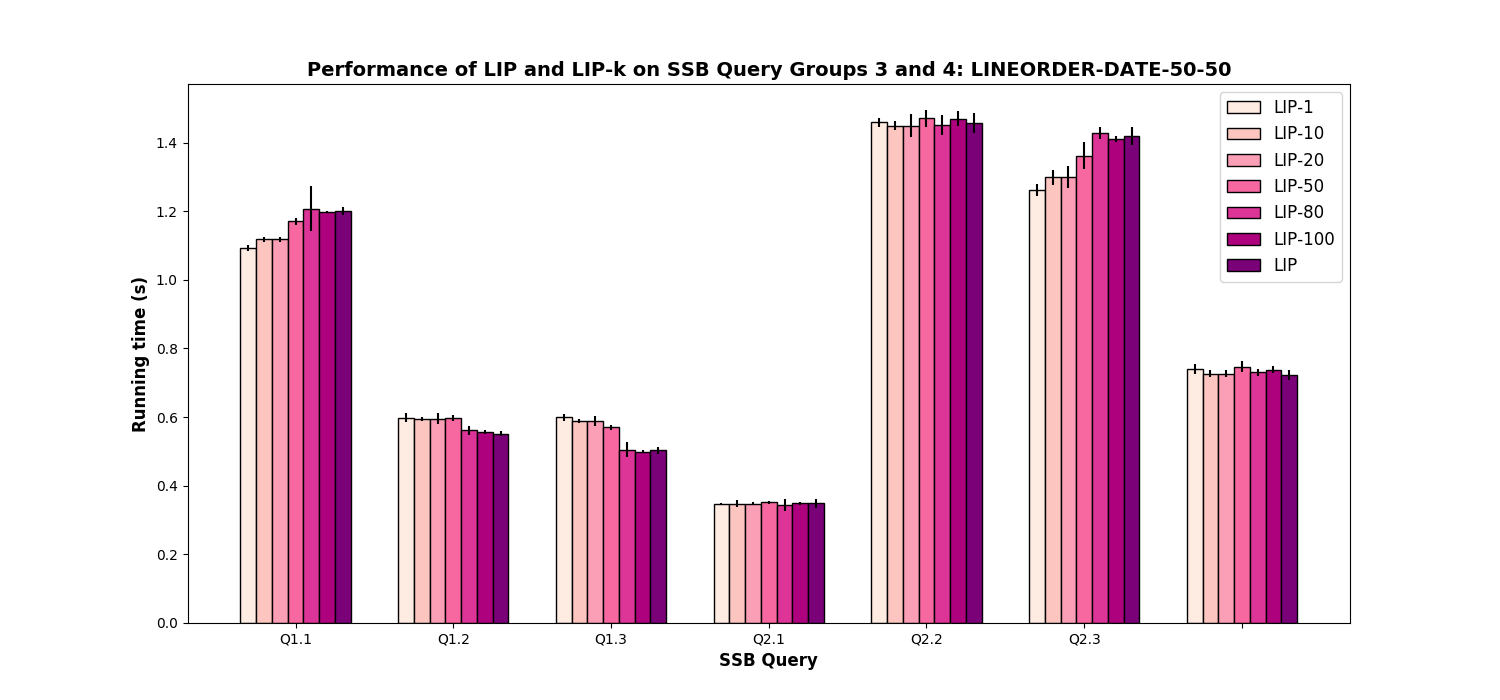
\includegraphics[width=0.9\textwidth,keepaspectratio]{lip-and-lipk-date-50-50}
    }
    \caption{Execution time for SSB query groups 3 and 4 on (a) \texttt{LINEORDER-DATE-FIRST-HALF} and (b)~\texttt{LINEORDER-DATE-50-50}}
    \label{fig:times1}
\end{figure}


\begin{figure}
    \centering    
    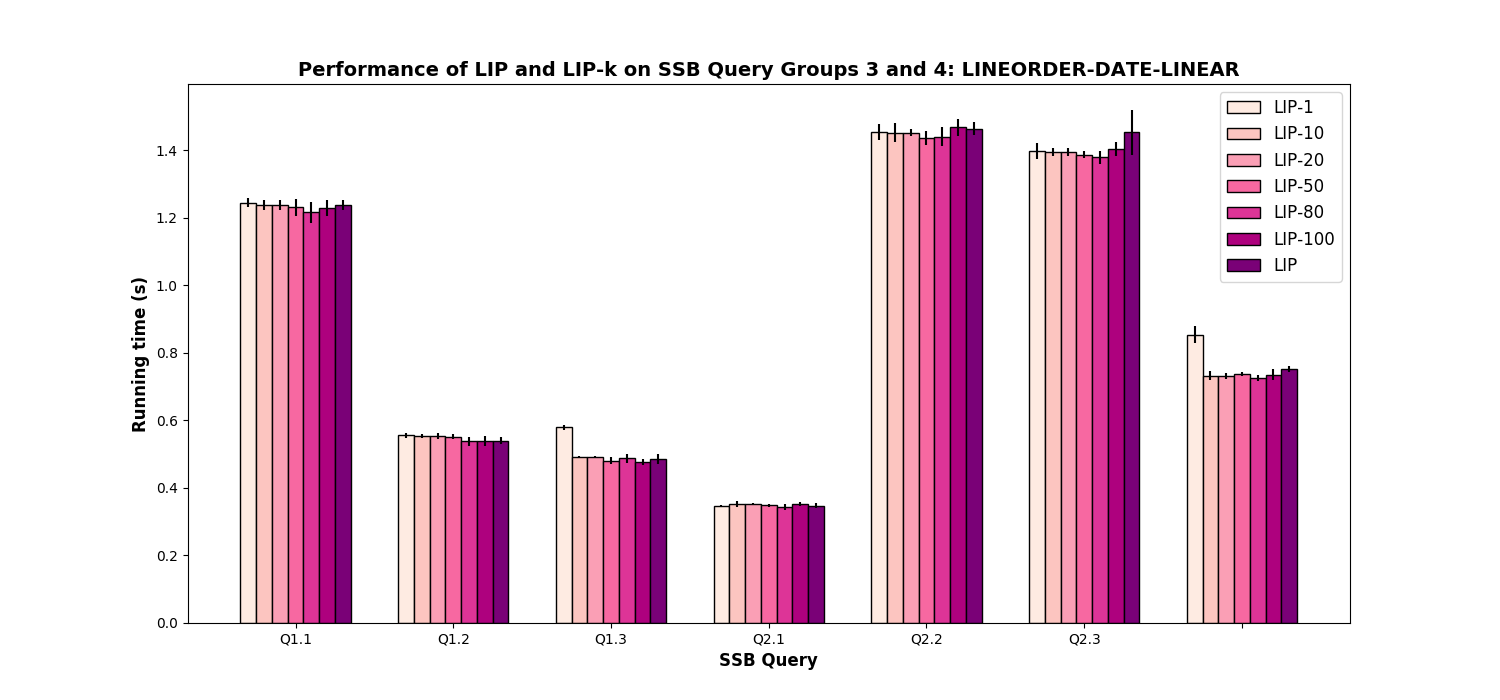
\includegraphics[width=0.9\textwidth,keepaspectratio]{lip-and-lipk-date-linear}
    \caption{Execution time for SSB query groups 3 and 4 on \texttt{LINEORDER-DATE-LINEAR}}
    \label{fig:times2}
\end{figure}

SSB query groups 1 and 2 do not join on \texttt{ORDER DATE}, 
and thus their execution times are unaffected by the skewed key column. 
Fig.~\ref{fig:times0}(a) shows execution times for these queries on the \texttt{LINEORDER-DATE-50-50} table.
As expected, we observe that LIP and LIP-$k$ have roughly equal performance for these queries.
Henceforth, we will exclude query groups 1 and 2 from our analysis, 
as they provide us no insight into the relative performance of LIP and LIP-$k$. 
Nevertheless, from these results, we see that the extra overhead associated with LIP-$k$ is negligible.

Query groups 3 and 4 --- except for query 4.1 --- join on \texttt{ORDER DATE}, 
so our skew can potentially affect the execution of LIP and LIP-$k$ on these queries.
Thus, we include only queries from groups 3 and 4 in our analysis. 
Query 4.1 is included as a "sanity check", since LIP and LIP-$k$ should have roughly equal performance on this query.

Fig.~\ref{fig:times0}(a) shows execution times for these queries on the \texttt{LINEORDER-UNIFORM} table.
We see that LIP-$1$ performs worse than all other algorithms on queries 3.3 and 4.3.
because it does not compute an accurate selectivity estimate using only one previous batch.
Otherwise, there is little difference between LIP and LIP-$k$ on uniform data.

Fig.~\ref{fig:times1}(a) shows execution times using \texttt{LINEORDER-DATE-FIRST-HALF}. 
We see that LIP and LIP-$k$ have roughly equal performance on queries 3.2, 3.3, 3.4, and 4.3 (in addition to 4.1).
In such queries, we do not gain much by responding to local changes in the key distribution,
since there exists another filter, {\it e.g.} the \texttt{SUPPLIER} filter, that is very selective. 
LIP generally will not notice when $\sigma_i^{\texttt{DATE}} = 0$ 
and instead applies the \texttt{SUPPLIER} filter first.
We observe that it is ``good enough" to apply a very selective filter first, even if it is not optimal.
On the other hand, LIP-$k$ performs better on queries 3.1 and 4.2, 
since the other filters in these queries are not particularly selective. 
We also observe that smaller $k$ has slightly better performance, 
because small $k$ can respond much more quickly to the sudden change in selectivity.

Fig.~\ref{fig:times1}(b) shows execution times using \texttt{LINEORDER-DATE-50-50}. 
LIP-$k$ performs better than LIP on queries 3.1 and 4.2 for the same reasons state in the preceding paragraph.
However, LIP performs better than LIP-$k$ on queries 3.2 and 3.3.
The key observation is that LIP-$k$ must first ``miss" before it can respond to a sudden change in selectivity.
When the batch selectivity for the \texttt{DATE} column switches from 0 to 1, 
the \texttt{DATE} filter appears first in the filter sequence, 
and thus LIP-$k$ performs an entire batch of unnecessary probes
before recognizing that the \texttt{DATE} filter should not be probed first.
We see that there is an inherent cost associated with responsiveness that may outweigh its benefit. 
% For example, consider LIP-1 processing the $101^{st}$ batch in \texttt{LINEORDER-DATE-50-50}. 
% At this point, the \text{DATE} filter has selectivity 0, and is thus probed first. 
% However, the \texttt{DATE} filter eliminates no tuples in the current batch, since the current batch has selectivity 1.
% Hence, LIP-1 performs an entire batch of unnecessary probes. 
% Afterwards, LIP-1 then knows to push the \texttt{DATE} filter to end of the filter sequence. 

Fig.~\ref{fig:times2} shows execution times using \texttt{LINEORDER-DATE-LINEAR}. 
LIP and LIP-$k$ have roughly the same performance for most queries, 
suggesting that both algorithms can adequately respond to smooth changes in key distributions.
Again, LIP-$1$ performs worse than all other algorithms on queries 3.3 and 4.3.
because of its inaccurate selectivity estimates.

\subsection{Competitive Ratio}
\label{sec:ratio}

To empirically support \ref{thm:det-n}, we construct an adversarial dataset which forces LIP to perform the maximum number of filter probes possible.
We now show how to generally construct such a dataset where two dimension tables are joined with the fact table ($n = 2$), mimicking the proof of Theorem \ref{thm:det-n}.

Suppose we are joining our fact table with two dimension tables A and B using LIP.
Let $f_i^A$ denote the selectivity of the Bloom filter for A after processing the $i^{th}$ batch. 
Let $\sigma_i^A$ denote the selectivity of the Bloom filter for A on the $i^{th}$ batch alone. 
Define analogous quantities for dimension table B.

We start with the first fact table batch having
$\sigma_1^A = \frac{1}{2} - \varepsilon$ and $\sigma_1^B = \frac{1}{2} + \varepsilon$ where $0 < \varepsilon < \frac{1}{2}$. Then for all $j > 1$, we let

\begin{equation*}
\sigma_j^A = 
    \begin{cases}
    1 & \text{if $j$ is even} \\[0.5em]
    0 & \text{if $j$ is odd} \\
    \end{cases} \quad \text{and }
\sigma_j^B = 
    \begin{cases}
    0 & \text{if $j$ is even} \\[0.5em]
    1 &  \text{if $j$ is odd} \\
    \end{cases}
\end{equation*}

Thus, the optimal filter sequence $S^{OPT}$ for $j > 1$ is 

\begin{align*}
S^{OPT} &= 
    \begin{cases}
    (B, A) & \text{if $j$ is even} \\[0.5em]
    (A, B) & \text{if $j$ is odd} \\
    \end{cases}\\[0.5em]
\end{align*}

\DeclarePairedDelimiter\floor{\lfloor}{\rfloor}
After processing batch $j > 1$, we have 
$f_j^A = \frac{\frac{1}{2} - \varepsilon + \floor{\frac{j}{2}}}{j}$ 
and 
$f_j^B = \frac{\frac{1}{2} + \varepsilon + \floor{\frac{j}{2}}}{j}$  
which can be rewritten as

\begin{equation*}
f_j^A = 
    \begin{cases}
    \frac{1}{2} + \frac{\frac{1}{2}-\varepsilon}{j} & \text{if $j$ is even} \\[0.5em]
    \frac{1}{2} - \frac{\varepsilon}{j} &  \text{if $j$ is odd} \\
    \end{cases}  \quad \text{and }
f_j^B = 
    \begin{cases}
    \frac{1}{2} - \frac{\frac{1}{2}-\varepsilon}{j} & \text{if $j$ is even} \\[0.5em]
    \frac{1}{2} + \frac{\varepsilon}{j} &  \text{if $j$ is odd} \\
    \end{cases}\\[0.5em]
\end{equation*}

Since $\frac{1}{2} - \varepsilon > 0$, LIP's filter ordering for $j > 1$ will be

\begin{align*}
S &= 
    \begin{cases}
    (A, B) & \text{if $j$ is even} \\[0.5em]
    (B, A) & \text{if $j$ is odd} \\
    \end{cases}\\[0.5em]
\end{align*}

which is the reverse of $S^{OPT}$. 
Hence, after the first batch has been processed, LIP will have worst-case performance on all remaining batches. 
As the number of batches in the fact table increases, the competitve ratio of LIP on such a dataset approaches $n =2$.

Following this construction, we generated an adversarial dataset for SSB query 4.2 with A = \texttt{DATE} and B = \texttt{PART},
excluding the joins on the \texttt{CUSTOMER} and \texttt{SUPPLIER} dimension tables.
We exclude these two joins because it is much simpler to generate an adversarial dataset on fewer dimension tables.
\footnote{In our implementation, we do not explicitly exclude the joins on \texttt{CUSTOMER} and \texttt{SUPPLIER} in query 4.2. 
Rather, we generate the adversarial dataset such that $\sigma_i^{\texttt{CUSTOMER}}=1$ and $\sigma_i^{\texttt{SUPPLIER}}=1$ for every batch $i$.
This achieves the same effect as excluding the joins.}

We ran LIP and LIP-$k$ on the uniform and adversarial datasets and computed the competitive ratio of each algorithm.
The results are depicted in Figure \ref{fig:cr}. 

\begin{figure}
    \centering
    \subfloat[]{
        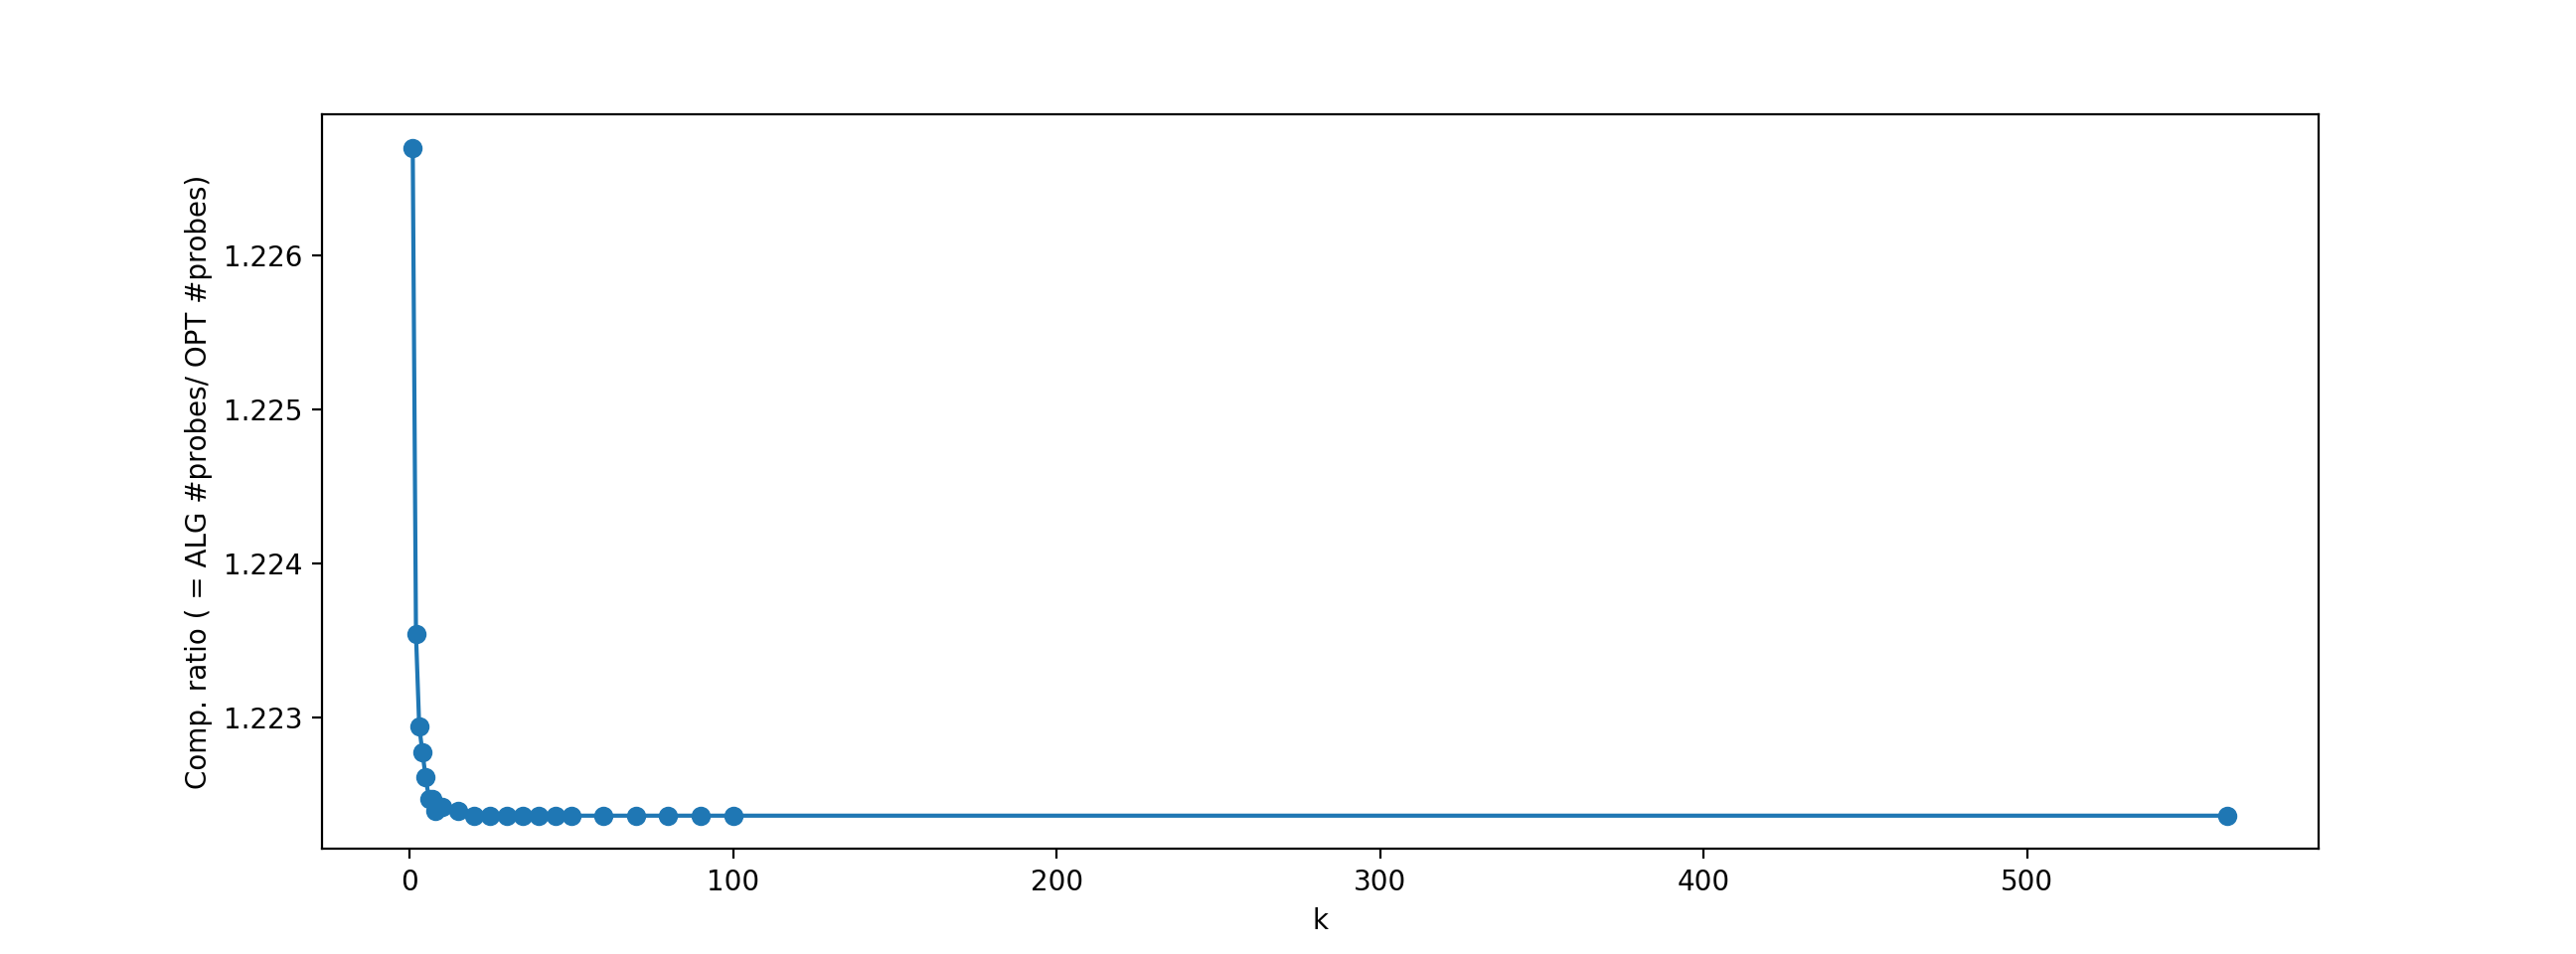
\includegraphics[width=0.9\textwidth,keepaspectratio]{cr-wide}
        %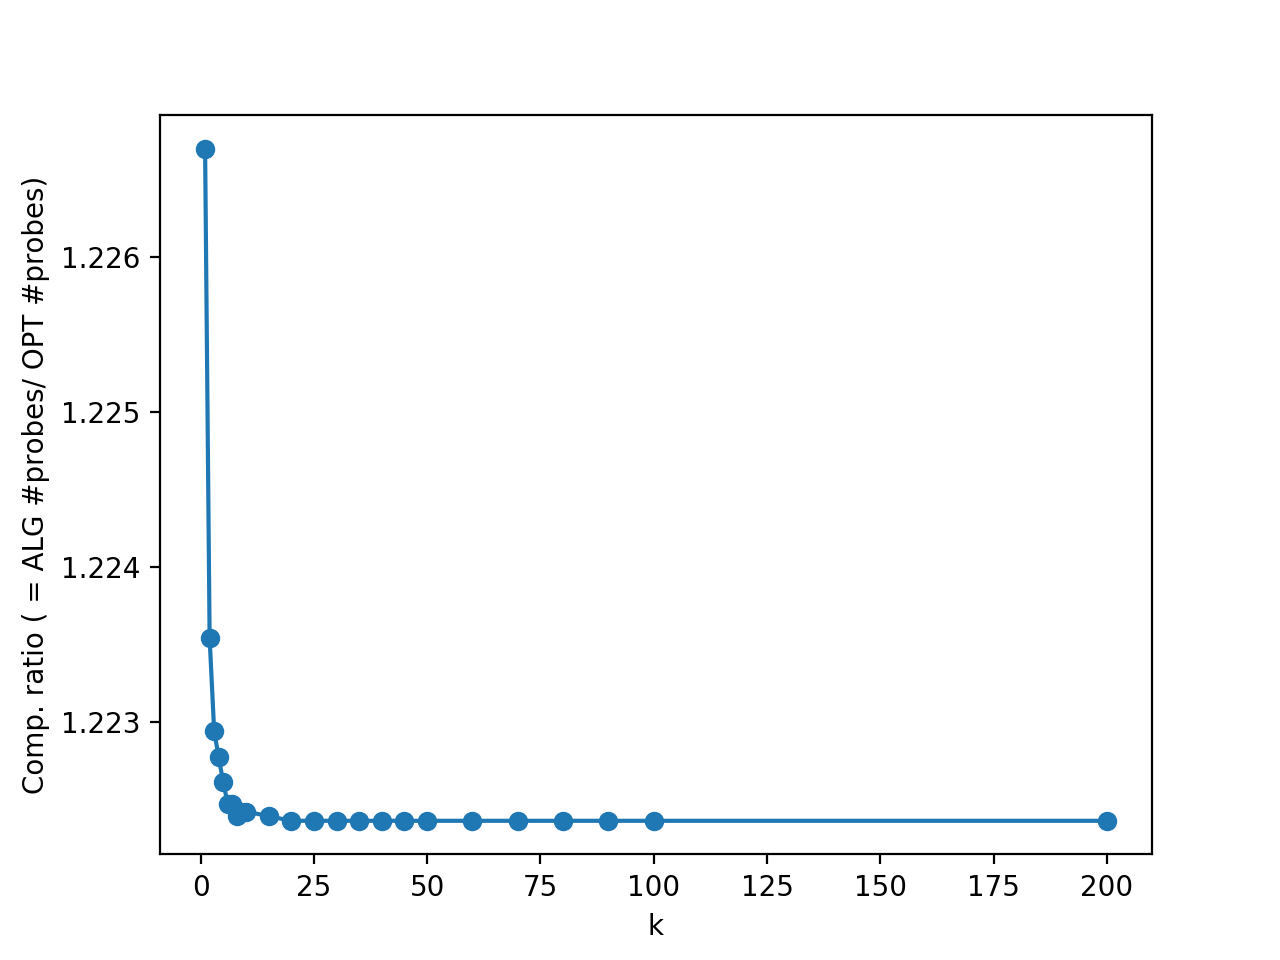
\includegraphics[width=0.9\textwidth,keepaspectratio]{cr-k-uniform}
    }   

    \quad
    
    \subfloat[]{
        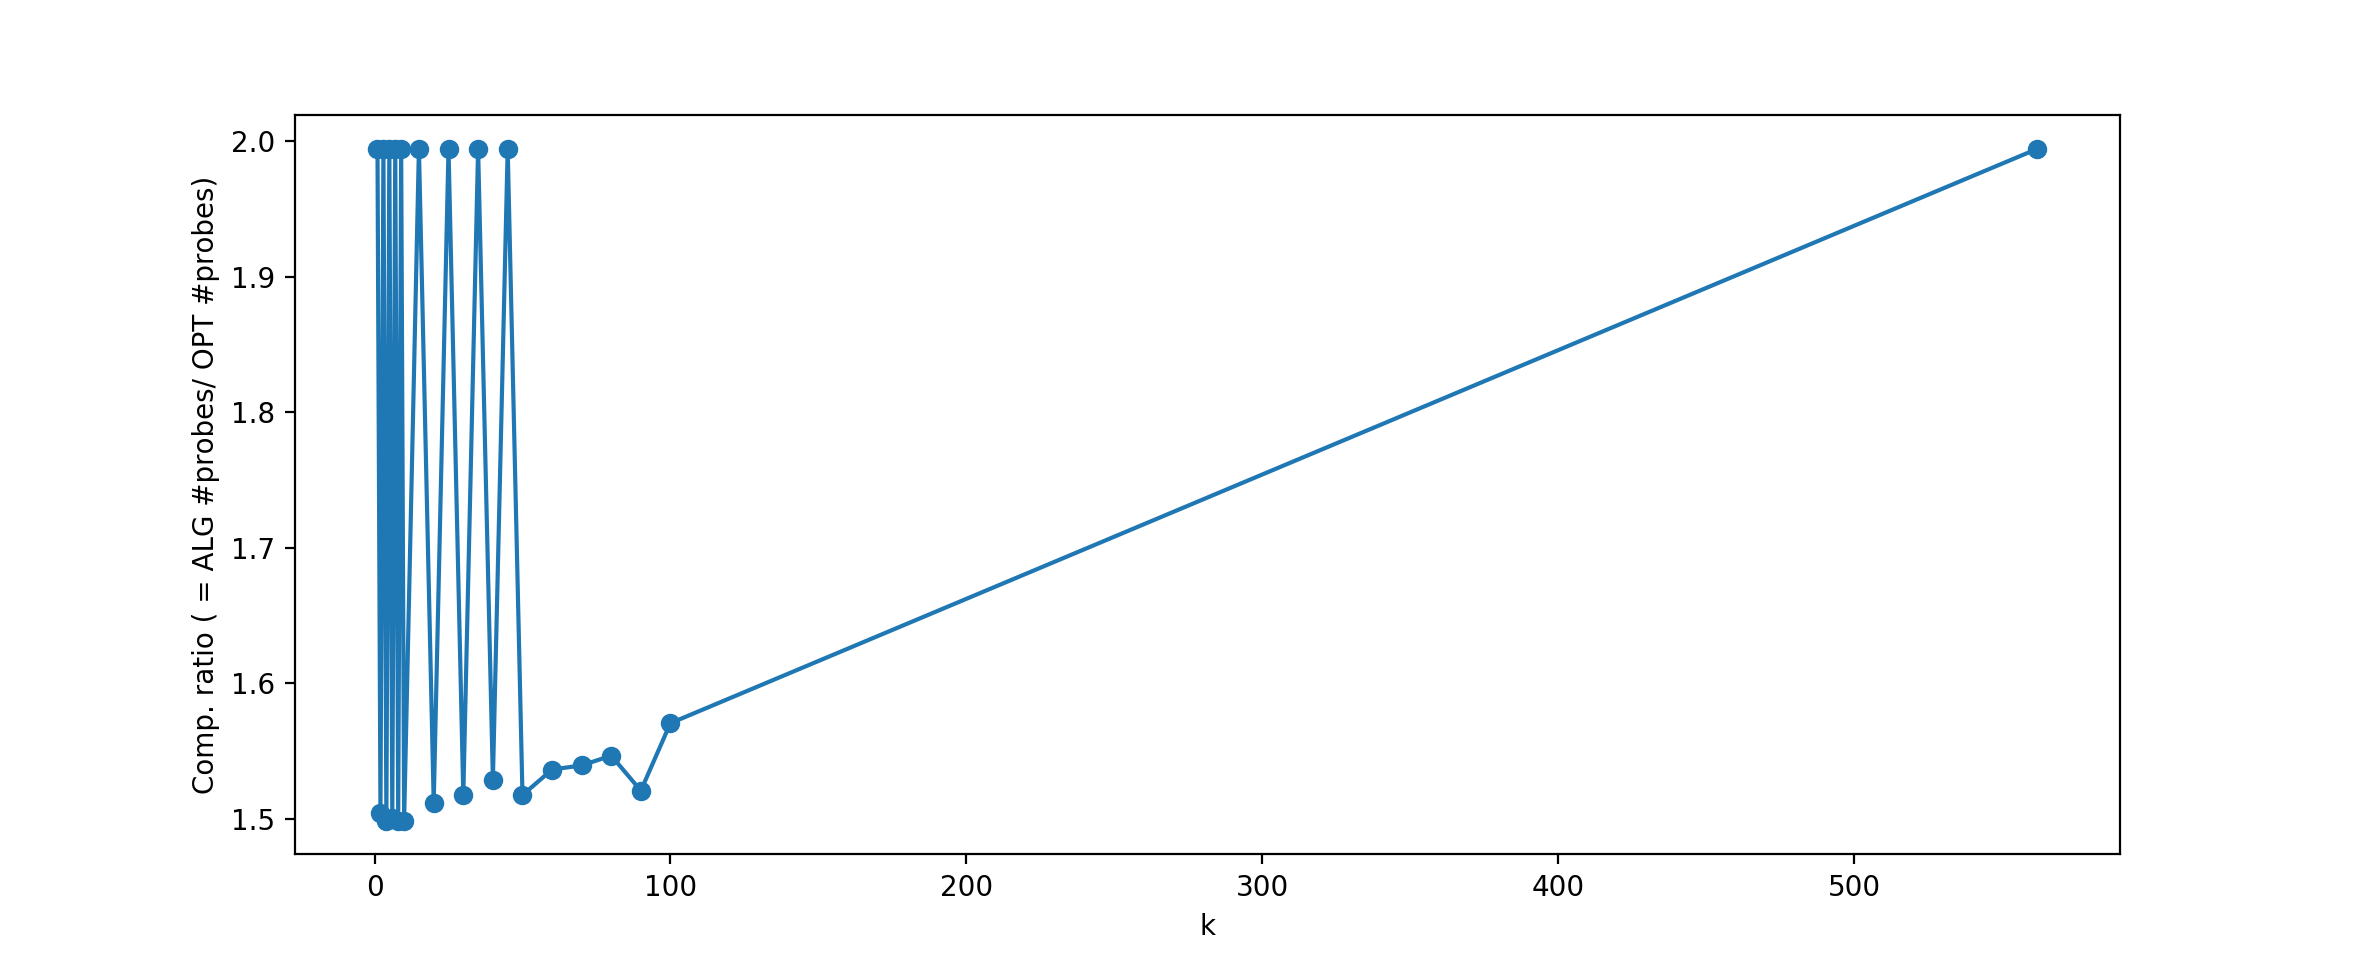
\includegraphics[width=0.9\textwidth,keepaspectratio]{cr-adversary-wide}
        %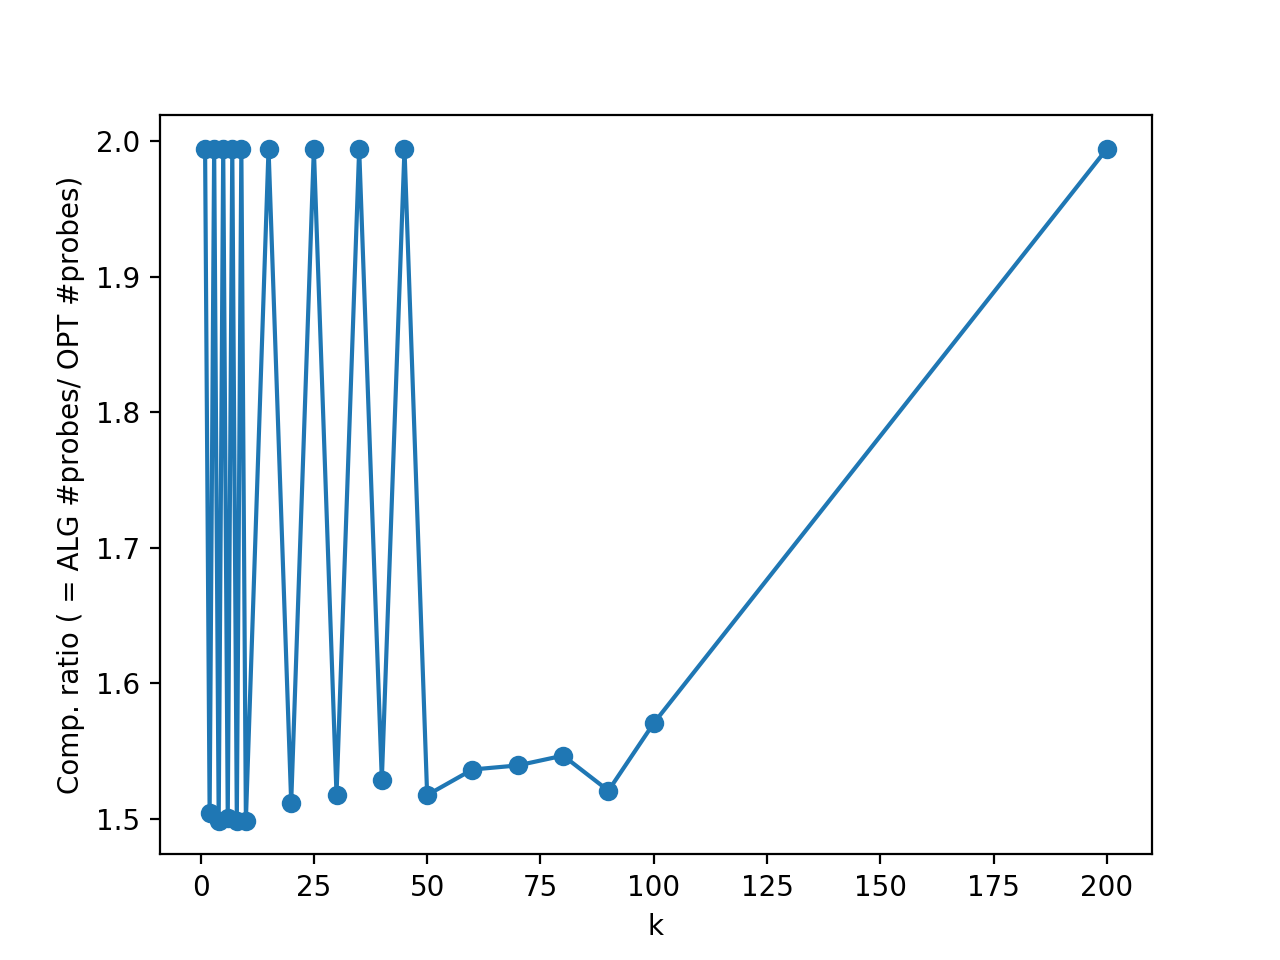
\includegraphics[width=0.9\textwidth,keepaspectratio]{cr-k-skewed}
    }
    \caption{The competitive ratios of LIP-$k$ against different $k$ values. We ran LIP-$k$ on uniform and adversarial datasets to produce (a) and (b) respectively. We plot $k = 1, 2, 3, 4, 5, 10, 15, 20, 25, 30, 35, 40, 45, 50, 60, 70, 80, 90, 100, 562$. The data point at $k = 562$ represents LIP (which is essentially LIP-$\infty$).}
    \label{fig:cr}
\end{figure}

When the keys in the fact table columns are distributed uniformly, the filters need not react to the local changes. LIP-$k$ with higher $k$produces a more accurate estimate of the selectivities than the LIP-$k$ with smaller $k$. Hence, the competitive ratio decreases slightly as $k$ increases, as depicted in Figure \ref{fig:cr}.

%@TODO: Explain the adversarial case using epsilons
Figure \ref{fig:cr}(b) displays how an adversarial dataset can make LIP-$k$ and LIP perform poorly. 
First, observe that LIP ({\it i.e.} LIP-562) achieves a competitive ratio of nearly 2.
Our modified query 4.2 has two joins, and thus the performance of LIP matches the worst case competitive ratio. 

LIP-$k$ with odd $k$ also achieves a competitive ratio of almost 2. 
For odd $k$, LIP-$k$'s selectivity estimates always contains one more odd (or even) batch than the other, 
and thus the estimated selectivity and filtering sequence are in favor of the majority batch type,
which produces the worst-case filter sequence on the following batch.

For even $k$, LIP-$k$'s selectivity estimates contain an equal amount of even an odd batches,  
and thus estimated selectivities remain the same ($1/2$ by construction) throughout the execution, 
and the filter sequence does not change. Thus for at most half of the batches it is optimal, 
and for the other half it is worse, 
resulting in a competitive ratio of at least \[ \frac{1 \times 1/2 + 2 \times 1/2}{1} = 1.5,\] as depicted in Figure \ref{fig:cr}. 

When $i \leq k$, LIP and LIP-$k$ execute identically, since LIP-$k$ has not yet ``forgotten" any previous batches. 
Thus, when $i \leq k$, LIP-$k$ achieves a competitive ratio of 2 on each batch, regardless of wheter $k$ is even or odd.
When $i > k$ and $k$ is odd, LIP-$k$ still achieves a competitive ratio of 2 on each batch.
However, When $i > k$ and $k$ is even, LIP-$k$ forgets to first batch and achieves a competive ratio of 1.5 on the remaining batches.
This explains why the competitive ratio increases for even $k$ as $k$ increases.
\footnote{An astute observer might notice that the competitive ratio decreases for $k = 50$ and $k = 90$. This is because the batch size is not constant throughout execution (see Section~\ref{sec:implementation}).}


%$k = 1, 2, 3, 4, 5, 10, 15, 20, 25, 30, 35, 40, 45, 50, 60, 70, 80, 90, 100$ on 